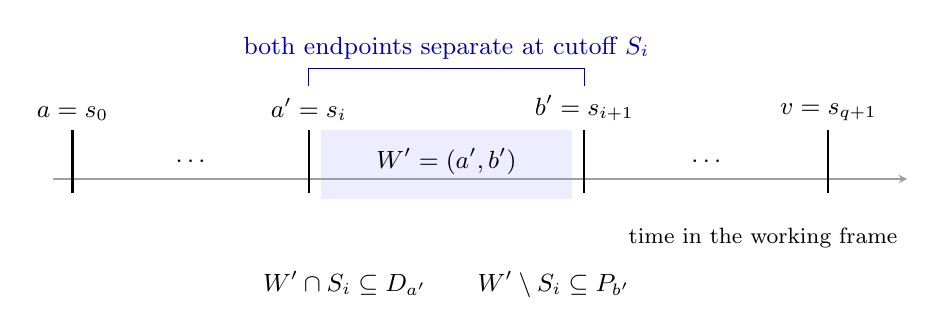
\begin{tikzpicture}[x=1cm,y=1cm,font=\small,>=stealth]
  \fill[blue!7] (3.15,-.25) rectangle (6.35,.62);
  \draw[->,gray!75] (-.25,0) -- (10.6,0);
  \node[anchor=east,font=\footnotesize] at (10.6,-.75)
    {time in the working frame};
  \foreach \x in {0,3,6.5,9.6}
    {\draw[thick] (\x,-.18) -- (\x,.62);}
  \node[above] at (0,.62) {$a=s_0$};
  \node[above] at (3,.62) {$a'=s_i$};
  \node[above] at (6.5,.62) {$b'=s_{i+1}$};
  \node[above] at (9.6,.62) {$v=s_{q+1}$};
  \node at (4.75,.22) {$W'=(a',b')$};
  \node at (1.5,.22) {$\cdots$};
  \node at (8.05,.22) {$\cdots$};
  \draw[blue!65!black] (3,1.18) -- (3,1.4) -- (6.5,1.4) -- (6.5,1.18);
  \node[above,text=blue!65!black] at (4.75,1.4)
    {both endpoints separate at cutoff $S_i$};
  \node[anchor=north,align=center] at (4.75,-1.05)
    {$W'\cap S_i\subseteq D_{a'}$\qquad
     $W'\setminus S_i\subseteq P_{b'}$};
\end{tikzpicture}
